\documentclass[11pt]{article}

\usepackage{a4wide}
\usepackage{hyperref}
\usepackage{mathptm}
\usepackage{xspace}
\usepackage{amsmath}
\usepackage{graphicx}
\usepackage{algorithm}
\usepackage{algpseudocode}
\usepackage{tikz}
\usepackage{tkz-graph}
\usetikzlibrary{shapes.misc, positioning}
\usepackage{listings}
\usepackage{color}
\usepackage{hyperref}

\definecolor{dkgreen}{rgb}{0,0.6,0}
\definecolor{gray}{rgb}{0.5,0.5,0.5}
\definecolor{mauve}{rgb}{0.58,0,0.82}

\lstset{frame=tb,
  language=Java,
  aboveskip=3mm,
  belowskip=3mm,
  showstringspaces=false,
  columns=flexible,
  basicstyle={\small\ttfamily},
  numbers=left,
  numberstyle=\tiny\color{gray},
  keywordstyle=\color{blue},
  commentstyle=\color{dkgreen},
  stringstyle=\color{mauve},
  breaklines=true,
  breakatwhitespace=true,
  tabsize=3
}
\begin{document}

%\input{commands}

\begin{titlepage}
\label{cover}
    \centering
    {\Huge \textbf{FeedApp}\par} 
    \vspace{2cm} 

    \begin{figure}[h!]
        \centering
        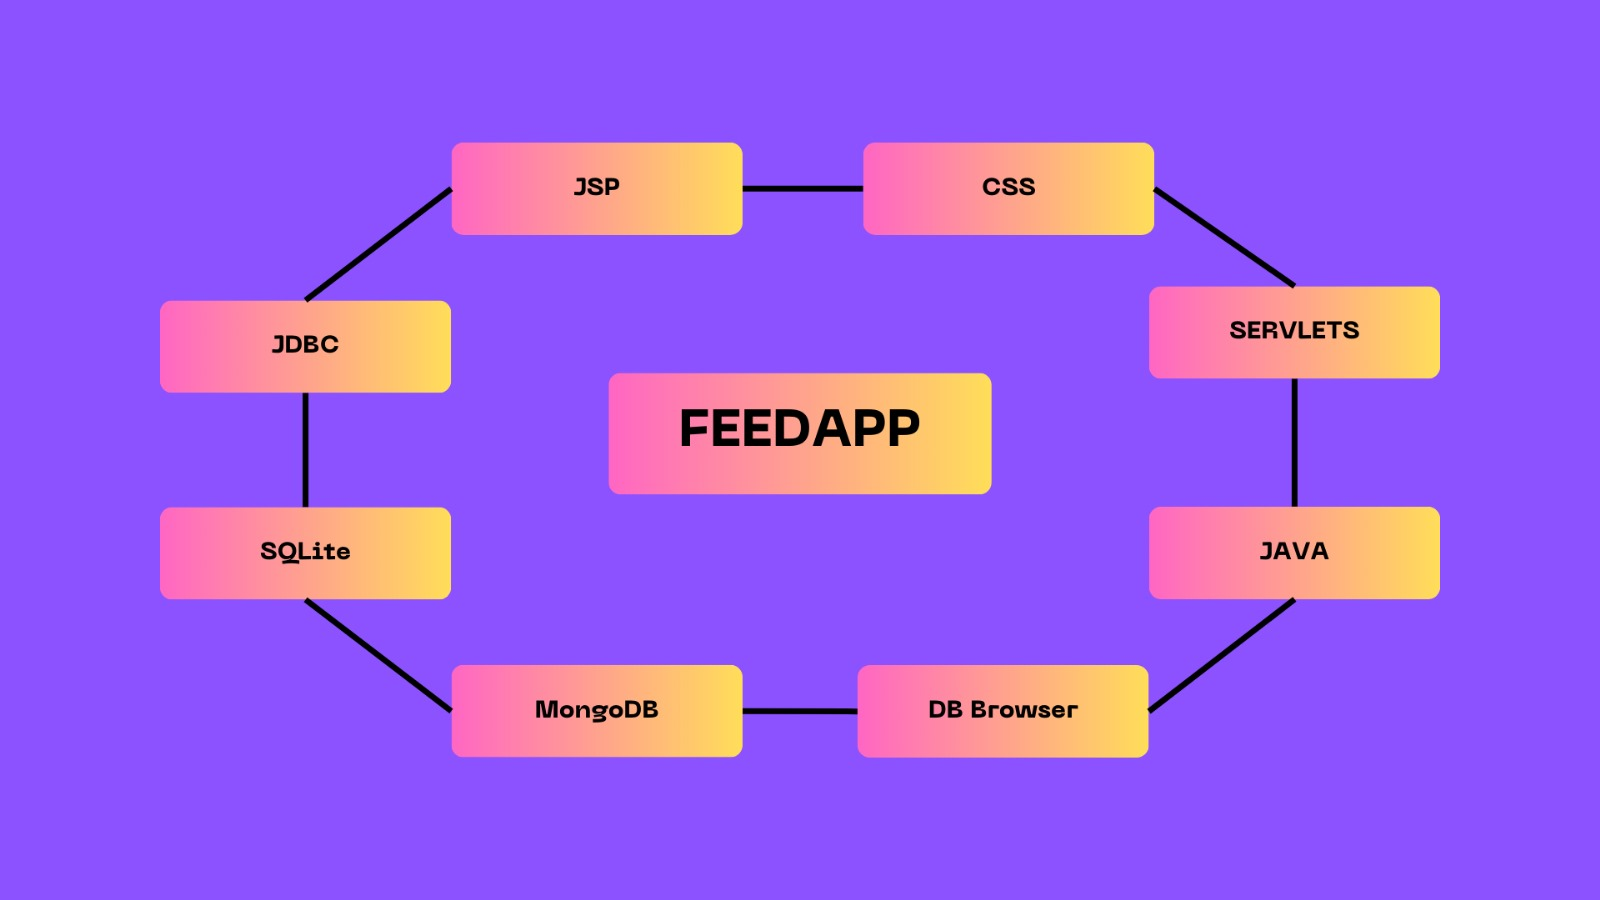
\includegraphics[width=0.8\textwidth]{figs/cover.jpg}  
    \end{figure}

    \vspace{2cm} 
    \noindent
    \textbf{Group 14:} \\
    Rafael Guiberteau Tinoco \\
    Darío Álvarez Barrado \\
    Ignacio Alcalde Torrescusa \\
    Carlos Fernández Calderón
\end{titlepage}

\begin{center}
    {\LARGE \textbf{INDEX}\par} 
    \vspace{2cm} 
\end{center}

\noindent
1. \textbf{\nameref{introduction}} \dotfill \pageref{introduction} \\
2. \textbf{\nameref{feedapp_design}} \dotfill \pageref{feedapp_design} \\
3. \textbf{\nameref{featured_technology}} \dotfill \pageref{featured_technology} \\
4. \textbf{\nameref{prototype_details}} \dotfill \pageref{prototype_details} \\
5. \textbf{\nameref{conclusion}} \dotfill \pageref{conclusion}

\vspace{3cm} 
\newpage 

\section{Introduction}
\label{introduction}

In this project, we explore a variety of software development technologies by developing a prototype application, \textbf{FeedApp}. Our aim is to gain hands-on experience with modern technologies and evaluate their effectiveness in creating a scalable, secure, and maintainable software solution. \textbf{FeedApp} serves as a testbed for understanding the strengths and trade-offs of different tools and frameworks, allowing us to conduct a comparative analysis based on real implementation outcomes.

\textbf{FeedApp} is structured to manage users, polls, and votes through a REST API, incorporating essential features such as authentication, persistent storage, and real-time messaging. These components not only fulfill the application's functional requirements but also facilitate a comprehensive assessment of each technology's role and efficiency.

In this report, we document our design decisions, technology choices, and their impact on the development process. Additionally, we introduce a "featured technology" that enhances the system, allowing for a deeper analysis of its integration and performance within the \textbf{FeedApp} ecosystem. This report, therefore, serves as both a record of our prototype's implementation and an evaluation of the technologies applied, highlighting the insights and lessons we gained as a team.

\newpage % Salto de página para el contenido siguiente

\section{FeedApp Design}
\label{feedapp_design}

In this section, we dive into designing \textbf{FeedApp}, including everything from the full process, idea formulation and ideation to the final iteration of the application. We would like to keep it as a straight number section. Hence it would be split into two important heads: \textbf{Use Cases, Domain and Architecture}.

\subsection{Use Cases}

Here are some examples of the key features of \textbf{FeedApp}:

\begin{itemize}
    \item \textbf{Create Poll:} Users can create a new poll by entering a question and the options to vote for.\\
    \textit{Example:} A teacher uses a poll to get feedback on the most effective teaching methods.
    
    \item \textbf{Edit Poll:} Users can update the details of polls they have created, such as the question or voting options.\\
    \textit{Example:} A poll creator modifies the options of a poll to include a new choice.
    
    \item \textbf{Delete Poll:} Users can remove their own polls from the system, which also deletes associated votes.\\
    \textit{Example:} A user removes a poll once this is no longer valid since the end of the poll.
    
    \item \textbf{Vote on Poll:} Registered users can select a voting option in a poll.\\
    \textit{Example:} A student votes on the schedule of their preferred study group.
    
    \item \textbf{View Results:} Users can view aggregated poll results, either in real-time or after the poll closes.\\
    \textit{Example:} A user checks which option received the highest votes in a class poll.
    
    \item \textbf{Register and Log In:} New users can register for an account, and existing users can log in to access personalized features.\\
    \textit{Example:} A student logs into their account to participate in new polls.
    
    \item \textbf{Edit Vote:} Users can change their vote before the poll closes.\\
    \textit{Example:} A user initially selects "Option A" but later changes to "Option B" after reconsidering.
    
    \item \textbf{View Profile:} Users can review their activity, such as the polls they created and the votes they cast.\\
    \textit{Example:} A poll creator views the list of their active and closed polls.
    
    \item \textbf{Log Out:} Users can securely end their session.
\end{itemize}

The diagram below visually represents how users interact with \textbf{FeedApp}:

\begin{figure}[thb]
	\centering
	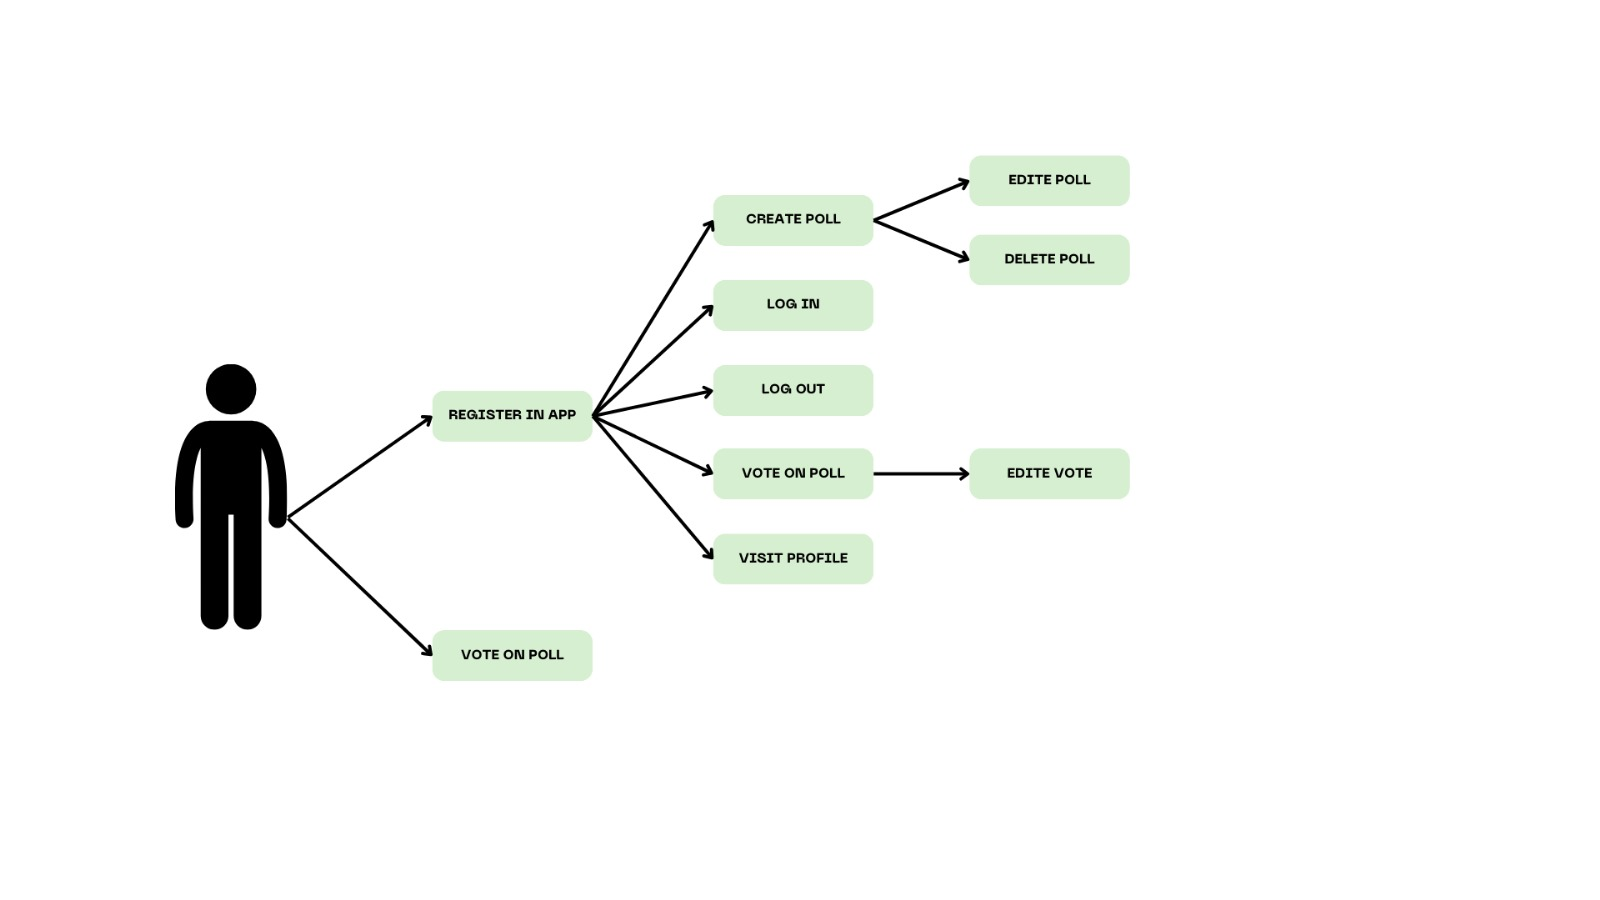
\includegraphics[scale=0.5]{figs/usecases.jpg}
	\caption{User interaction diagram for FeedApp.}
	\label{fig:feedapp_diagram}
\end{figure}


\subsection{Domain}

The \textbf{FeedApp} domain model underpins the business logic and data structure, defining the core entities and their relationships. This ensures a structured and scalable design.

\subsubsection{Key Entities}

\begin{enumerate}
    \item \textbf{User}
    \begin{itemize}
        \item \textbf{Relationships:}
        \begin{itemize}
            \item A user can create multiple polls.
            \item A user can participate in multiple votes.
        \end{itemize}
        \item \textbf{Description:} This class represents individuals interacting with the system as creators or participants in polls.
    \end{itemize}
    
    \item \textbf{Poll}
    \begin{itemize}
        \item \textbf{Attributes:}
        \begin{itemize}
            \item \texttt{id (Integer):} A unique identifier.
            \item \texttt{title (String):} The poll title.
            \item \texttt{question (String):} Refers to the poll question.
            \item \texttt{createdAt (Instant):} Creation timestamp.
            \item \texttt{validUntil (Instant):} Expiration timestamp.
            \item \texttt{user\_id (Integer):} Creator's identifier.
        \end{itemize}
        \item \textbf{Relationships:}
        \begin{itemize}
            \item The poll belongs just to one user.
            \item Can contain multiple vote options.
            \item Can have multiple associated votes.
        \end{itemize}
        \item \textbf{Description:} Is a central entity linking questions, options, and participants.
    \end{itemize}
    
    \item \textbf{VoteOption}
    \begin{itemize}
        \item \textbf{Attributes:}
        \begin{itemize}
            \item \texttt{id (Integer):} A unique identifier.
            \item \texttt{caption (String):} Option description.
            \item \texttt{presentationOrder (Integer):} Display order.
            \item \texttt{poll\_id (Integer):} Associated poll.
        \end{itemize}
        \item \textbf{Relationships:}
        \begin{itemize}
            \item Each VoteOption belongs to one poll.
            \item It’s linked to multiple votes.
        \end{itemize}
        \item \textbf{Description:} Represents all the choices available for users to select in a poll.
    \end{itemize}
\end{enumerate}


\subsubsection{Vote}

\begin{itemize}
    \item \textbf{Attributes:}
    \begin{itemize}
        \item \texttt{id (Integer):} A unique identifier.
        \item \texttt{votedAt (Instant):} Vote timestamp.
        \item \texttt{user\_id (Integer):} Voter's identifier.
        \item \texttt{voteOption\_id (Integer):} Selected option.
    \end{itemize}
    \item \textbf{Relationships:}
    \begin{itemize}
        \item Each vote is made by one user.
        \item Each vote is linked to one vote option.
    \end{itemize}
    \item \textbf{Description:} Captures voting activity, storing the user's choice in a poll.
\end{itemize}

\subsubsection{Key Relationships}

\begin{itemize}
    \item \textbf{User $\leftrightarrow$ Poll (1:N):} Each user can create multiple polls, but a poll belongs to one user.\\
    \textit{Example:} A teacher creates several polls for different courses.

    \item \textbf{Poll $\leftrightarrow$ VoteOption (1:N):} A poll can have multiple vote options, allowing users to provide various responses.\\
    \textit{Example:} A poll on favorite programming languages includes options like "Python," "Java," and "C++."

    \item \textbf{Poll $\leftrightarrow$ Vote (1:N):} A poll can receive multiple votes, reflecting participant responses.\\
    \textit{Example:} Students vote on their preferred class schedule.

    \item \textbf{VoteOption $\leftrightarrow$ Vote (1:N):} Each vote is tied to a specific option within a poll.
\end{itemize}

\subsubsection{UML Class Diagram}

\begin{figure}[h!]
    \centering
    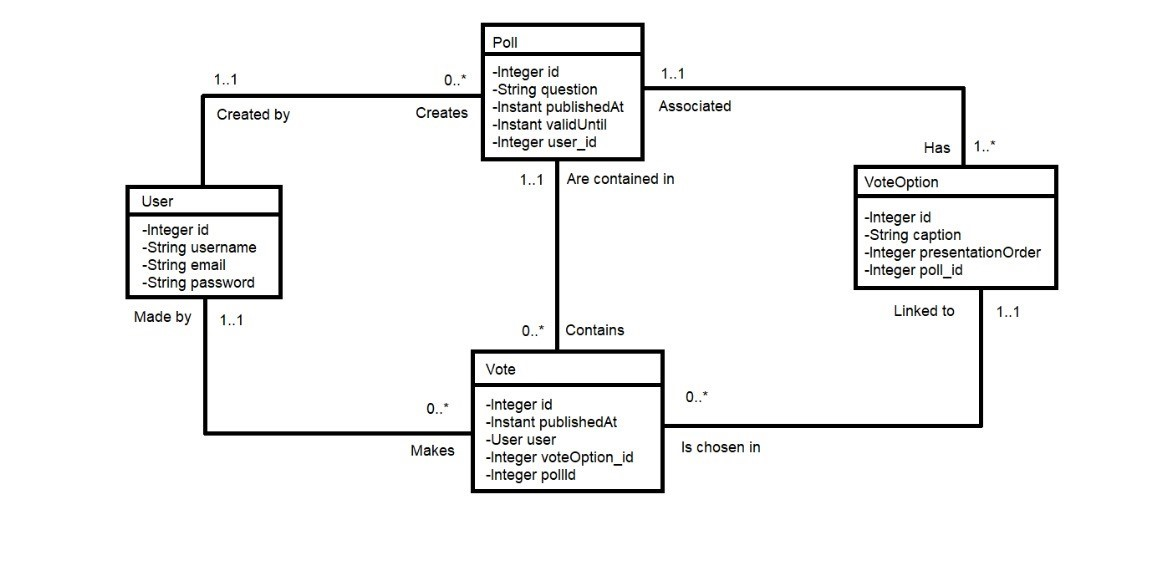
\includegraphics[width=0.9\textwidth]{figs/uml_diagram.jpg} 
    \caption{UML Class Diagram for FeedApp}
    \label{fig:uml_class_diagram}
\end{figure}

The UML diagram visualizes these relationships and cardinalities, ensuring that FeedApp's business logic is both intuitive and maintainable.


\subsection{Architecture}

This domain model was selected to ensure flexibility, scalability, and integrity.

\subsubsection{Choosing Technologies}

\begin{itemize}
    \item \textbf{Frontend:} JSP and CSS for interface creation and styling.
    \begin{itemize}
        \item \textbf{JSP (JavaServer Pages):} Technology for creating dynamic web pages by combining HTML and Java logic, enabling interactive interfaces.
        \item \textbf{CSS:} Style sheet language used to customize the appearance of web pages, enhancing the visual user experience.
        \item \textbf{JavaScript:} Programming language used to add interactive features like animations (confetti, loaders) and dynamic modals to improve user engagement.
    \end{itemize}

    \item \textbf{Backend:} Java servlets for business logic.
    \begin{itemize}
        \item \textbf{Java Servlets:} Java components that handle server-side requests, enabling backend logic for dynamic web applications.
    \end{itemize}

    \item \textbf{Database:} SQLite for structured data storage and MongoDB for dynamic data handling.
    \begin{itemize}
        \item \textbf{JDBC (Java Database Connectivity):} API for efficient interaction between Java applications and relational databases like SQLite.
        \item \textbf{SQLite:} An efficient relational database to organize your structured data with well-defined relationships employing primary and foreign keys.
        \item \textbf{MongoDB:} A NoSQL database commonly known for its use of Semi-Structured data, useful to store application statistics.
    \end{itemize}

    \item \textbf{Data Analysis \& Communication:} Real-time data integration and management with RabbitMQ.
    \begin{itemize}
        \item \textbf{RabbitMQ:} A messaging system that allows application components to communicate in real time and process asynchronously.
    \end{itemize}
\end{itemize}

\subsubsection{Development Highlights}

\begin{figure}[h!]
    \centering
    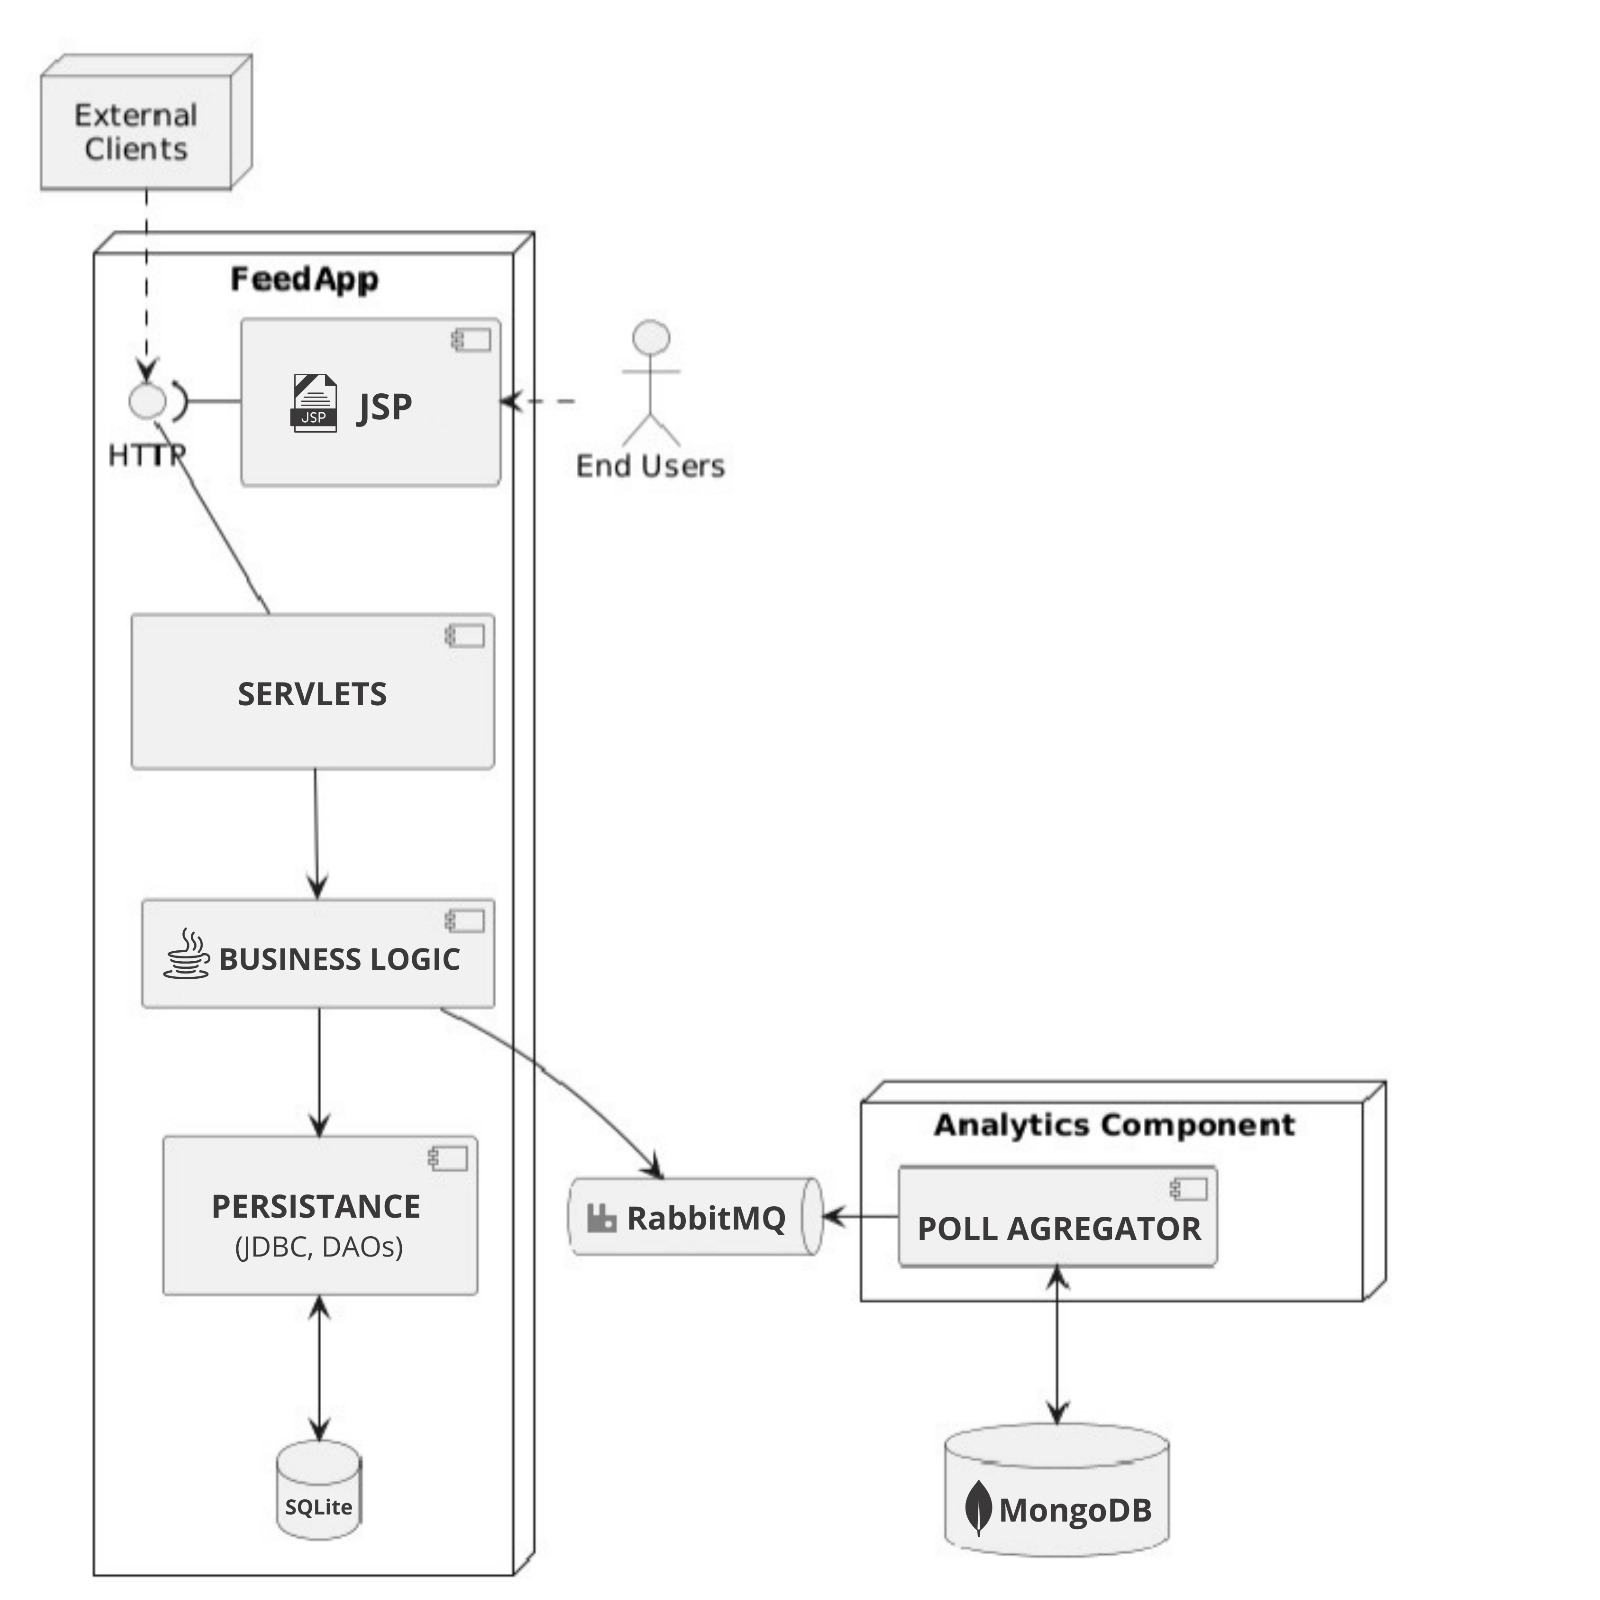
\includegraphics[width=0.9\textwidth]{figs/architecture_diagram.jpg} 
    \caption{Development Highlights Diagram for FeedApp}
    \label{fig:development_highlights}
\end{figure}

Here is the description of how each component communicates in the workflow:

\begin{enumerate}
    \item \textbf{External Clients:}
    \begin{itemize}
        \item End users interact with the application via HTTP requests, which are routed to the \textbf{FeedApp}.
    \end{itemize}

    \item \textbf{FeedApp:}
    \begin{itemize}
        \item \textbf{JSP:} Frontend layer. It receives user input (over HTTP) and creates dynamic web pages in return to the users. SERVLETS communicate directly with JSP.
        \item \textbf{SERVER SIDE COMPONENTS: SERVLETS:} It is a controller. It gets requests coming from the front end (JSP); it processes them and sends requests to the BUSINESS LOGIC layer.
        \item \textbf{BUSINESS LOGIC:} This is the application core. It handles the data obtained through SERVLETS and communicates with the PERSISTENCE layer to perform database-related actions.
        \item \textbf{PERSISTENCE:} Use of JDBC and DAOs to perform CRUD (Create, Read, Update, Delete) operations on the \textbf{SQLite} database.
    \end{itemize}

    \item \textbf{SQLite:}
    \begin{itemize}
        \item Serves as the primary database, storing structured data such as user information, polls, and votes. It is accessed through the PERSISTENCE layer.
    \end{itemize}

    \item \textbf{RabbitMQ:}
    \begin{itemize}
        \item Acts as a message broker between the \textbf{FeedApp} and the \textbf{Analytics Component}.
        \item After critical events (e.g., poll creation or vote submission), BUSINESS LOGIC publishes messages to RabbitMQ to update analytics asynchronously.
    \end{itemize}

    \item \textbf{Analytics Component:}
    \begin{itemize}
        \item The \textbf{Poll Aggregator} receives messages from RabbitMQ and updates the statistics in \textbf{MongoDB}, which stores semi-structured data like user counts, polls created, and votes recorded.
    \end{itemize}

    \item \textbf{MongoDB:}
    \begin{itemize}
        \item A NoSQL database that holds analytics and semi-structured data enabling the system to manage large-scale and dynamic data efficiently.
    \end{itemize}
\end{enumerate}

\section{Featured Technology in Use}
\label{featured_technology}

\subsection{Introduction}

The project focuses on developing a robust and scalable web application by integrating foundational and modern technologies. Key technologies included \textbf{Java Servlets} for backend development, \textbf{JSP} and \textbf{CSS} for the frontend, and \textbf{SQLite} and \textbf{MongoDB} for data management. Additionally, \textbf{RabbitMQ} was integrated to manage real-time updates and communication.

One of the critical decisions in the development process was choosing \textbf{Java Servlets} over \textbf{Spring Boot annotations} for backend functionality. Both technologies offer distinct advantages, but the selection of Servlets was influenced by several factors, including the project’s scope, team expertise, and the need for a lightweight approach.

This analysis examines the rationale behind this choice, comparing the strengths, weaknesses, and use cases of Servlets and Spring Boot annotations. Understanding this comparison provides deeper insights into the trade-offs involved in backend technology selection, especially for small- to medium-scale projects.

\subsection{Genealogy and Context of the Problem Domain}

\subsubsection{2.1 History and Evolution of Java Servlets}
Introduced in the late 1990s as part of Java EE, Servlets addressed inefficiencies of CGI scripts by offering a thread-based model for dynamic, server-side web applications. Over time, they evolved to integrate with JavaBeans, JDBC, and modern frameworks.

\subsubsection{2.2 History and Evolution of Spring Boot Annotations}
Spring Boot, launched in 2014, simplified enterprise Java development through features like dependency injection and annotation-driven configurations (e.g., \texttt{@RestController}, \texttt{@Autowired}). Its modular, abstraction-heavy approach accelerates development for large-scale applications.

\subsubsection{2.3 Application Domains}
\begin{itemize}
    \item \textbf{Java Servlets:} Best for small- to medium-scale projects needing low-level control and performance.
    \item \textbf{Spring Boot:} Ideal for enterprise-grade, scalable, and modular applications.
\end{itemize}

\subsubsection{2.4 Initial Comparison: Goals of Servlets and Spring Boot}
\begin{itemize}
    \item \textbf{Servlets:} Provide a lightweight, foundational framework for handling HTTP requests and responses. Focus on performance, simplicity, and educational value.
    \item \textbf{Spring Boot:} Abstract complexities, enabling faster development of scalable, enterprise-grade applications. Focus on modularity, automation, and ease of use.
\end{itemize}

\begin{table}[h!]
    \centering
    \begin{tabular}{|l|l|l|}
        \hline
        \textbf{Feature} & \textbf{Servlets} & \textbf{Spring Boot Annotations} \\
        \hline
        Ease of use & Manual coding, more control. & Simplified with abstractions. \\
        \hline
        Learning Curve & Lower, core Java concepts. & Higher, requires Spring knowledge. \\
        \hline
        Performance & Minimal overhead. & Some overhead, better scalability. \\
        \hline
        Scalability & Suitable for small projects. & Optimized for large systems. \\
        \hline
        Development Speed & Slower due to manual setup. & Faster with automated tools. \\
        \hline
    \end{tabular}
    \caption{Comparison of Servlets and Spring Boot Annotations}
    \label{tab:servlet_springboot_comparison}
\end{table}

\subsection{Hypothesis and Experiment Design}

\subsubsection{Hypothesis}
The hypothesis explores whether Java Servlets are a better fit for small-scale projects compared to Spring Boot, focusing on performance, simplicity, and faster development setup for basic functionality.

\subsection{Hypothesis and Experiment Design}

\subsubsection{Hypothesis}

The hypothesis for this experiment is:

\begin{quote}
    \textit{"Java Servlets offer greater efficiency and are better suited for small-scale projects compared to Spring Boot annotations, particularly in terms of performance, development simplicity, and scalability for limited concurrent users."}
\end{quote}

This hypothesis stems from the belief that Servlets, due to their lightweight nature and direct handling of HTTP requests, are more efficient for straightforward projects with minimal complexity. Conversely, Spring Boot's abstraction layers, while beneficial for large-scale or modular applications, could introduce unnecessary overhead in a smaller context.

\subsubsection{Experiment Description}

To validate this hypothesis, a simple web application feature---a login form---was implemented using both Java Servlets and Spring Boot annotations. This feature involved processing HTTP POST requests, validating user credentials, and generating appropriate responses. The following aspects were tested:

\begin{enumerate}
    \item \textbf{Functionality Evaluated}
    \begin{itemize}
        \item \textbf{Form Handling:} Both implementations processed login credentials submitted via an HTML form.
        \item \textbf{Session Management:} Verified user sessions were properly managed after successful login.
        \item \textbf{Database Interaction:} Each implementation connected to a SQLite database to retrieve and validate user data.
    \end{itemize}

    \item \textbf{Metrics Analyzed}
    \begin{itemize}
        \item \textbf{Performance:} Measured response time under varying levels of concurrent user requests.
        \item \textbf{Development Simplicity:} Evaluated the amount of boilerplate code and configuration required for each technology.
        \item \textbf{Scalability:} Tested how well each technology handled an increasing number of concurrent users.
        \item \textbf{Error Handling:} Assessed how each implementation dealt with invalid input or failed database connections.
    \end{itemize}

    \item \textbf{Tools Used for Testing}
    \begin{itemize}
        \item \textbf{Apache JMeter:} Simulated concurrent user requests to measure response time and throughput.
        \item \textbf{SQLite:} Used as the database for credential storage to ensure consistency across both implementations.
        \item \textbf{Code Complexity Analysis:} Compared lines of code and configuration effort between Servlets and Spring Boot.
    \end{itemize}

    \item \textbf{Experimental Setup}
    \begin{itemize}
        \item \textbf{Environment:} Both implementations were deployed on a local Tomcat server for consistency.
        \item \textbf{User Load:} Tests included 1, 50, 100, and 500 concurrent users to evaluate scalability.
        \item \textbf{Timeframe:} Each test scenario ran for 2 minutes with ramp-up times of 10 seconds.
    \end{itemize}
\end{enumerate}

\subsection{Quantitative Analysis}

\begin{enumerate}
    \item \textbf{Response Time Under Load}
    \begin{itemize}
        \item \textbf{Java Servlets:} Consistently performed better under low to moderate load (1--100 users), with average response times of 50ms for 1 user and 120ms for 100 users. Performance degraded slightly under heavy load (500 users), with response times reaching 300ms.
        \item \textbf{Spring Boot:} Exhibited higher response times at all levels, averaging 80ms for 1 user, 150ms for 100 users, and 400ms for 500 users. The additional overhead from the framework's abstractions likely contributed to this.
    \end{itemize}

    \item \textbf{Development Time}
    \begin{itemize}
        \item \textbf{Java Servlets:} Required more lines of code for request processing and session management, taking approximately 4 hours to fully implement the login feature.
        \item \textbf{Spring Boot:} With its annotation-based approach, implementation was faster, taking 2.5 hours.
    \end{itemize}

    \item \textbf{Scalability}
    \begin{itemize}
        \item \textbf{Java Servlets:} Handled up to 100 concurrent users efficiently but showed increased latency and dropped requests beyond this threshold.
        \item \textbf{Spring Boot:} Managed larger loads better, sustaining acceptable performance for up to 300 concurrent users, likely due to its optimized thread handling and built-in features.
    \end{itemize}
\end{enumerate}

\subsection{Qualitative Analysis}

\begin{enumerate}
    \item \textbf{Ease of Use}
    \begin{itemize}
        \item \textbf{Java Servlets:} Required a detailed understanding of the HTTP lifecycle, making development more time-intensive but offering granular control over request handling.
        \item \textbf{Spring Boot:} Simplified the process significantly with annotations like \texttt{@PostMapping} and \texttt{@SessionAttributes}, reducing boilerplate code.
    \end{itemize}

    \item \textbf{Development Experience}
    \begin{itemize}
        \item \textbf{Java Servlets:} Developers appreciated the educational value of working directly with core Java APIs, gaining a deeper understanding of web application mechanics.
        \item \textbf{Spring Boot:} Preferred by developers seeking faster results and focusing on business logic rather than infrastructure setup.
    \end{itemize}

    \item \textbf{Limitations Observed}
    \begin{itemize}
        \item \textbf{Java Servlets:}
        \begin{itemize}
            \item Lack of built-in features like validation or dependency injection increased development time.
            \item Manual configuration for session and error handling was error-prone.
        \end{itemize}
        \item \textbf{Spring Boot:}
        \begin{itemize}
            \item Introduced unnecessary overhead for a simple project.
            \item Required a learning curve for developers unfamiliar with the Spring ecosystem.
        \end{itemize}
    \end{itemize}
\end{enumerate}

\subsection{Reasons for Choosing Servlets in the Project}

\begin{itemize}
    \item \textbf{Simplicity and Alignment with Team Capabilities:} Java Servlets were chosen primarily due to their simplicity and directness, aligning perfectly with the team’s existing skill set. Unlike Spring Boot, which requires a deeper understanding of its ecosystem and configuration, Servlets offer a more straightforward approach to handling HTTP requests and responses. This was particularly beneficial given the project’s limited timeline and scope.

    \item \textbf{Educational Relevance:} One of the key objectives of the project was to strengthen the team’s foundational knowledge of backend development. By working with Servlets, the team gained hands-on experience in managing the request-response lifecycle, session handling, and database connectivity. These are essential skills for understanding the fundamentals of web application development and debugging.

    \item \textbf{Prior Experience with Servlets:} The team had prior experience using Java Servlets during a previous project at our home university, where we implemented a booking system. This familiarity with Servlets allowed us to leverage existing knowledge and focus on refining and optimizing our approach. This prior exposure ensured that the learning curve was minimal, allowing us to proceed confidently with the development process.

    \item \textbf{Project Needs and Technical Justification:} The project’s requirements—focused on implementing a lightweight and efficient web application—did not demand the advanced features provided by Spring Boot, such as dependency injection or modular microservices support. Servlets provided sufficient control and granularity to meet the functional needs of the project, including handling requests, managing user sessions, and interacting with a database.

    \item \textbf{Advantages of Servlets in This Case:} 
    \begin{itemize}
    \item \textbf{Low Overhead}: Servlets avoid the abstraction layers of Spring Boot, resulting in better performance for a small-scale application.
    \item \textbf{Granular Control}: They allowed the team to customize request handling and response formatting directly.
    \item \textbf{Seamless Integration}: Servlets integrate effortlessly with JDBC for database operations, which is crucial for implementing features like user authentication.
    \item \textbf{Simpler Deployment}: For environments limited to Java EE containers, deploying a Servlet-based application was less complex and more resource-efficient than setting up a Spring Boot environment.

  
\end{itemize}
\end{itemize}
\subsection{Integration of Servlets into the Prototype}

\subsubsection{Implementation of Core Functionality}

Servlets were used to build the backbone of the application, handling critical functionalities such as:

\begin{itemize}
    \item \textbf{User Authentication:} A Servlet processed login requests, validated credentials against a SQLite database, and managed user sessions.
    \item \textbf{Dynamic Content Rendering:} JSP pages were used in conjunction with Servlets to deliver dynamic content, creating an interactive user interface.
    \item \textbf{Request Handling:} Custom Servlets managed HTTP POST and GET requests, routing them to appropriate resources based on user input.
\end{itemize}

\subsubsection{Optimizations Made for Servlet-Based Solutions}

\begin{itemize}
    \item \textbf{Session Management:} Manual adjustments were made to optimize session handling, ensuring efficient memory usage and avoiding session conflicts during concurrent access.
    \item \textbf{Performance Enhancements:} Query optimization in the database layer and caching strategies were implemented to reduce latency.
    \item \textbf{Error Handling:} Custom error-handling Servlets were introduced to manage invalid inputs and database connection failures gracefully.
\end{itemize}

\subsubsection{Integration with Other Technologies}
To build a robust and scalable prototype, Servlets were integrated with complementary technologies:

\begin{itemize}
    \item \textbf{RabbitMQ:}Servlets interacted with RabbitMQ for asynchronous messaging, enabling real-time updates for certain application features.
    \item \textbf{JDBC:} Direct database connectivity was established using JDBC for operations like user authentication and data retrieval. Servlets acted as the middle layer between the client-side interface and the backend database.
    \item \textbf{Frontend Compontents:} The Servlets seamlessly rendered JSP pages, dynamically populating content based on user actions and database queries.
\end{itemize}

\section{Reflexive Comparison and Future Applications}

\subsection{1. When Spring Boot Would Be a Better Fit}

Although Servlets were appropriate for this project, Spring Boot offers clear advantages for certain scenarios:

\begin{itemize}
    \item \textbf{Enterprise-Scale Applications:} For large projects requiring modularity, scalability, and microservices architecture, Spring Boot's built-in features such as dependency injection and service discovery simplify development.
    \item \textbf{Rapid Development:} The automation provided by annotations like \texttt{@GetMapping} and \texttt{@Autowired} accelerates development, making it ideal for projects with tight deadlines.
    \item \textbf{Complex Integrations:} Spring Boot excels in managing advanced integrations, such as security layers (via Spring Security), distributed systems, and messaging queues, with minimal configuration.
    \item \textbf{Team Collaboration:} In larger teams, Spring Boot’s abstractions and ecosystem can improve productivity by standardizing development practices.
\end{itemize}

\subsection{2. Lessons Learned from Working with Servlets}

\begin{itemize}
    \item \textbf{Fundamental Understanding:} Developing with Servlets reinforced our knowledge of HTTP protocols, session management, and multithreading, which are critical for understanding backend operations.
    \item \textbf{Granular Control:} We learned the value of having fine-grained control over request-response handling, which was especially helpful in customizing the application to meet specific requirements.
    \item \textbf{Effort vs. Abstraction:} While Servlets provide full control, we recognized the trade-off in terms of the additional development effort required compared to frameworks like Spring Boot.
    \item \textbf{Manual Optimizations:} The project highlighted the challenges of optimizing session handling, error management, and scalability manually, tasks that Spring Boot simplifies significantly.
\end{itemize}

\subsection{3. Preparing for Spring Boot in Future Projects}

This project served as a stepping stone for transitioning to more advanced frameworks like Spring Boot. The following steps will guide our preparation:

\begin{itemize}
    \item \textbf{Learning the Ecosystem:} Familiarizing ourselves with key Spring components, such as Spring Data, Spring Security, and Spring Cloud, to leverage its full potential.
    \item \textbf{Experimentation:} Conducting smaller projects using Spring Boot to gain hands-on experience with annotations, dependency injection, and microservices.
    \item \textbf{Framework Evaluation:} Developing an understanding of when to use Spring Boot versus other tools, based on project size, complexity, and requirements.
\end{itemize}



\section{Prototype Details}
\label{prototype_details}

\subsection{Prototype Description}

We created a prototype for FeedApp, an interactive app to make polls and provide them with voting and management support. Below is the detailed flow of main system functionalities:

\subsubsection{Poll Creation Flow}
\begin{itemize}
    \item If a user doesn’t have an account, they can register one, while if they do have an account, they just have to log in with said account.
    \item After logging in, users will be taken to a page where all polls are displayed and will be able to create a new poll.
    \item When users create a poll, in the poll creation interface, they have to first provide the poll title.
    \item Upon entering the title, the user is then prompted in a second interface to add voting options.
    \item Finally, when confirmed, the poll with its options is stored in the database and is displayed in the poll listing page.
\end{itemize}

\subsubsection{Voting Flow}
\begin{itemize}
    \item Guests can view the polls and vote without an account. These votes will be saved in the database with \texttt{"user\_id"} set to null.
    \item If the user has voted on a poll, the identified users have the ability to change their vote. These updates are then instantly shown in the database as well as in the system user interface.
\end{itemize}

\subsubsection{Profile and Poll Management}
\begin{itemize}
    \item This will take authenticated users to their profile, with their registered details and a list of all polls they have created.
    \item Users can edit or delete existing polls from this section, as well as change the corresponding voting options.
\end{itemize}

\subsubsection{Analytical Reports}
\begin{itemize}
    \item Implemented a NoSQL database system (\textbf{MongoDB}) to store and query analytical data. These contain statistics on registered users, polls created, and votes cast (from both identified and unidentified users).
\end{itemize}

\subsection{Data Storage Considerations}

The prototype uses a hybrid approach to data storage, which consists of using a relational and NoSQL database:


\subsubsection{Relational Database (SQLite)}

\begin{itemize}
    \item A simple-to-use, serverless, self-contained, zero-configuration, cross-platform, file-based SQL database. It is most suitable for applications that have a well-defined structure and SQL queries.
    \item Stores core operational data (users, polls, vote choices, etc.).
    \item There are related tables included in the database structure:
    \begin{itemize}
        \item \textbf{Users:} Stores basic information about users (\texttt{id}, \texttt{username}, \texttt{email}, \texttt{password}).
        \item \textbf{Polls:} Stores the polls created by users.
        \item \textbf{VoteOptions:} Lists the options available for each poll.
        \item \textbf{Votes:} Logs each vote cast, including the \texttt{user\_id} if applicable.
    \end{itemize}
\end{itemize}

\subsubsection{NoSQL Database (MongoDB)}

\begin{itemize}
    \item A non-relational (NoSQL) database management system that stores information in JSON or BSON documents, providing flexibility in the structure of the data and making it ideal for handling large amounts of unstructured or semi-structured data.
    \item \textbf{What We Used It For:} To store analytical data, like:
    \begin{itemize}
        \item Total number of registered users.
        \item Number of polls created and their relation to users.
        \item Votes cast, distinguishing between identified and unidentified users.
    \end{itemize}
    \item \textbf{MongoDB collections include:}
    \begin{itemize}
        \item \textbf{Users:} User information for analysis.
        \item \textbf{Polls:} Statistics on created polls.
        \item \textbf{Votes:} Records of votes for participation analysis.
    \end{itemize}
\end{itemize}

Using a dual design isolates operational data from analytical data, allowing for greater performance and the ability to perform specific queries.

\newpage 



\section{Conclusion \& References}
\label{conclusion}

The development of FeedApp successfully integrated key technologies to create a functional and scalable application that efficiently manages polls and votes. Among the chosen technologies, \textbf{Java Servlets} stood out as the featured technology, providing detailed control over the system's logic and seamless handling of user requests. Servlets enabled the backend to efficiently process requests, interact with the persistence layer, and manage data flow across the application.

To complement Servlets, \textbf{RabbitMQ} played a supporting role in enabling asynchronous, real-time messaging for analytical data synchronization, while \textbf{SQLite} and \textbf{MongoDB} were utilized for data storage. This hybrid approach allowed SQLite to manage operational data efficiently and MongoDB to handle analytical data with flexibility and scalability.

For future improvements, adopting frameworks like \textbf{Spring Boot} could simplify backend management for more complex projects while enhancing the authentication system to improve security. Additionally, implementing advanced features such as interactive data visualizations for analytics could significantly boost the system's usability and provide more value to users.

Overall, this project established a robust foundation for further development while providing the team with valuable experience in utilizing modern technologies.

\subsection*{References}

\begin{itemize}
    \item Oracle Documentation: \textbf{``Java Servlet Technology''}: \url{https://docs.oracle.com/javaee/7/tutorial/servlets.htm}
    \item Mozilla Developer Network (MDN): \textbf{``CSS: Cascading Style Sheets''}: \url{https://developer.mozilla.org/en-US/docs/Web/CSS}
    \item Mozilla Developer Network (MDN): \textbf{``JavaScript Guide''}: \url{https://developer.mozilla.org/en-US/docs/Web/JavaScript/Guide}
    \item DB Browser for SQLite: \textbf{``Database Management Tool for SQLite''}: \url{https://sqlitebrowser.org/}
    \item MongoDB Documentation: \textbf{``Getting Started with MongoDB''}: \url{https://www.mongodb.com/docs/manual/}
    \item RabbitMQ Documentation: \textbf{``Messaging with RabbitMQ''}: \url{https://www.rabbitmq.com/documentation.html}
    \item Spring Boot Documentation: \textbf{``Spring Boot Reference Guide''}: \url{https://docs.spring.io/spring-boot/docs/current/reference/html/}
\end{itemize}

\subsection*{Github Link of the Project Code:}
\url{https://github.com/r4f4777/FeedApp/tree/main/Project%20Code }

\subsection*{Github Link of the SQL database:}
\url{https://github.com/r4f4777/FeedApp/tree/main/Databases }

\end{document}
